\usetikzlibrary{calc}
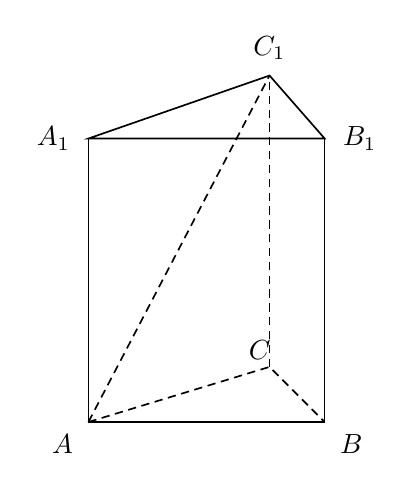
\begin{tikzpicture}[x=1cm,y=1cm,line width=.6pt,font=\normalsize]
\coordinate (A) at (0,0);
\coordinate (B) at (3,0);
\coordinate (C) at (2.3,0.7);
\coordinate (A1) at (0,3.6);
\coordinate (B1) at (3,3.6);
\coordinate (C1) at (2.3,4.4);
% front face solid
\draw (A) -- (B) -- (B1) -- (A1) -- cycle;
% top triangle solid
\draw (A1) -- (B1) -- (C1) -- cycle;
% hidden base + CC1 + diagonal AC1 dashed
\draw[densely dashed] (A) -- (C) -- (B);
\draw[densely dashed] (C) -- (C1);
\draw[densely dashed] (A) -- (C1);
% labels
\node[anchor=north east,xshift=-2pt,yshift=-1pt] at (A) {$A$};
\node[anchor=north west,xshift=2pt,yshift=-1pt] at (B) {$B$};
\node[anchor=south east,xshift=4pt,yshift=-1pt] at (C) {$C$};
\node[anchor=east,xshift=-3pt] at (A1) {$A_{1}$};
\node[anchor=west,xshift=3pt] at (B1) {$B_{1}$};
\node[anchor=south,yshift=2pt] at (C1) {$C_{1}$};
\end{tikzpicture}
